\documentclass[20pt,a1paper,landscape]{tikzposter}

% required packages
\usepackage{amsmath}
\usepackage{amsfonts}
\usepackage{graphicx}
\usepackage{natbib}
\usepackage{url}

%% Available themes: see also
%% https://bitbucket.org/surmann/tikzposter/downloads/themes.pdf
\usetheme{Default}
\colorlet{backgroundcolor}{white}

% title information
\title{Your Very Interesting Poster Title}
\author{First Author$^1$, Second author$^2$, Third Author$^1$}
\institute{$^1$University of California, Berkeley; $^2$ Other Institution}

% dictate default block options
\newcommand{\myblock}[2]{\block[titleinnersep=4mm, linewidth=1mm]{#1}{#2}}
\newcommand{\mysmallblock}[2]{\block[titleinnersep=1mm, linewidth=1mm]{{\small #1}}{{\small#2\par}}}

% compact bibliography
\renewcommand{\bibsection}{}
\setlength{\bibsep}{0pt plus 0.3ex}
\begin{document}

% title and graphics. increase the width to wrap around your poster title
\maketitle[width=17in]
\node[anchor=west] at (TP@title.west) {
\includegraphics[width=8cm]{logos/cal}};
\node[anchor=east] at (TP@title.east) {
\includegraphics[width=7cm]{logos/arxiv-link-qr-code}};

\begin{columns}

  \column{0.333}

  \myblock{Background}{
    \begin{itemize}
      \item Put your background information here.
      \item Bullet points make the content digestible.
      \item Only include salient details.
      \item Feel free to cite a few important references
        \citep{example-citation}.
      \item These boxes are resized automatically.
      \item Use \texttt{\textbackslash vspace\{\}} to alter the amount of
    white space above and below the text.
    \end{itemize}
  }

  \myblock{Statistical Problem Formulation}{
    Outline the statistical problem formulation of your topic using as little
    notation as possible. 
  }

  \column{0.334}
  
  \myblock{Inference}{
    Next, you can outline the inference procedure that you've proposed to solve
    your problem.

    \vspace{1em}

    \innerblock[]{Interesting Result}{
      If you'd like to present an important theorem or lemma, or want
      to call attention to an interesting fact, then you can highlight it with
      a sub-box.
    }

  }

  \myblock{Simulation Study}{
    If you performed any numerical experiments, present them here. Here's an
    example. Try to avoid too much text, if any. If anyone has questions, you
    can answer them directly.

    \vspace{0.25em}

    \begin{center}
      \begin{tikzfigure}
        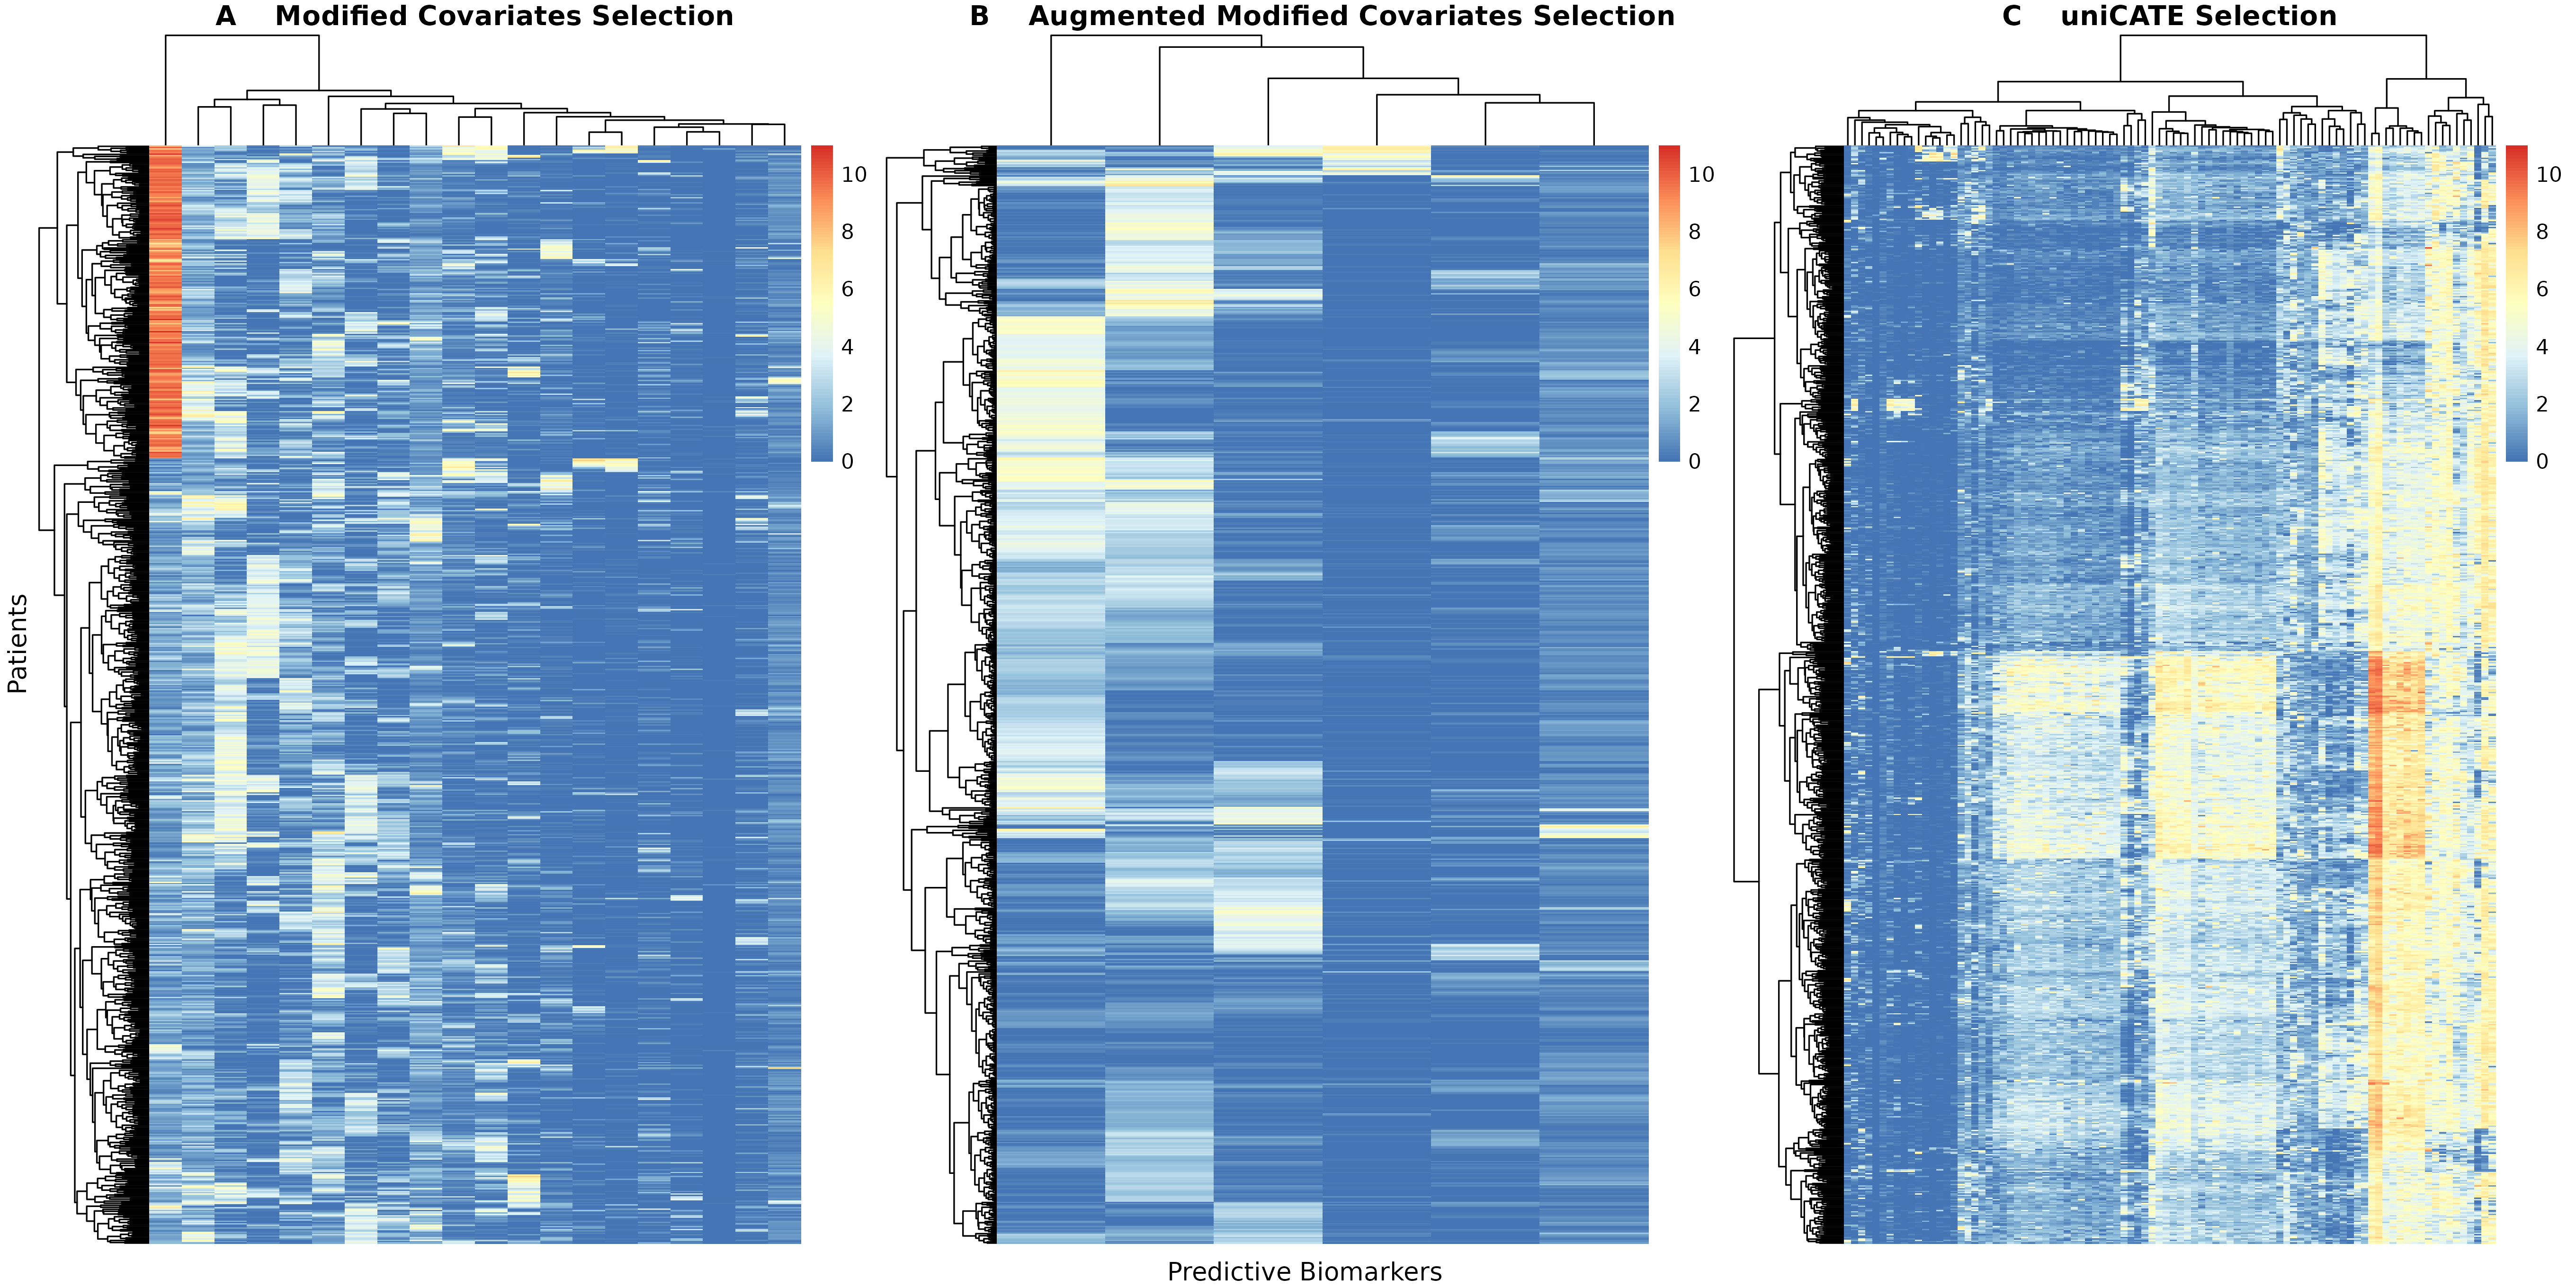
\includegraphics[width=0.295\textwidth]{figures/heatmaps.png}
      \end{tikzfigure}
    \end{center}
  }
  
  \mysmallblock{Funding}{
    \vspace{-1.5em}
    Don't forget to thank your funding sources! You can also use this box
    for acknowledgements by modifying the box title.
    \vspace{-2em}
  }
  
  \column{0.333}

  \myblock{Application}{
    Include the results of your real-data application here, if any. Again, try
    not to include too much text. Let the figure(s) speak for themselves.

    \vspace{0.25em}

    \begin{center}
      \begin{tikzfigure}
        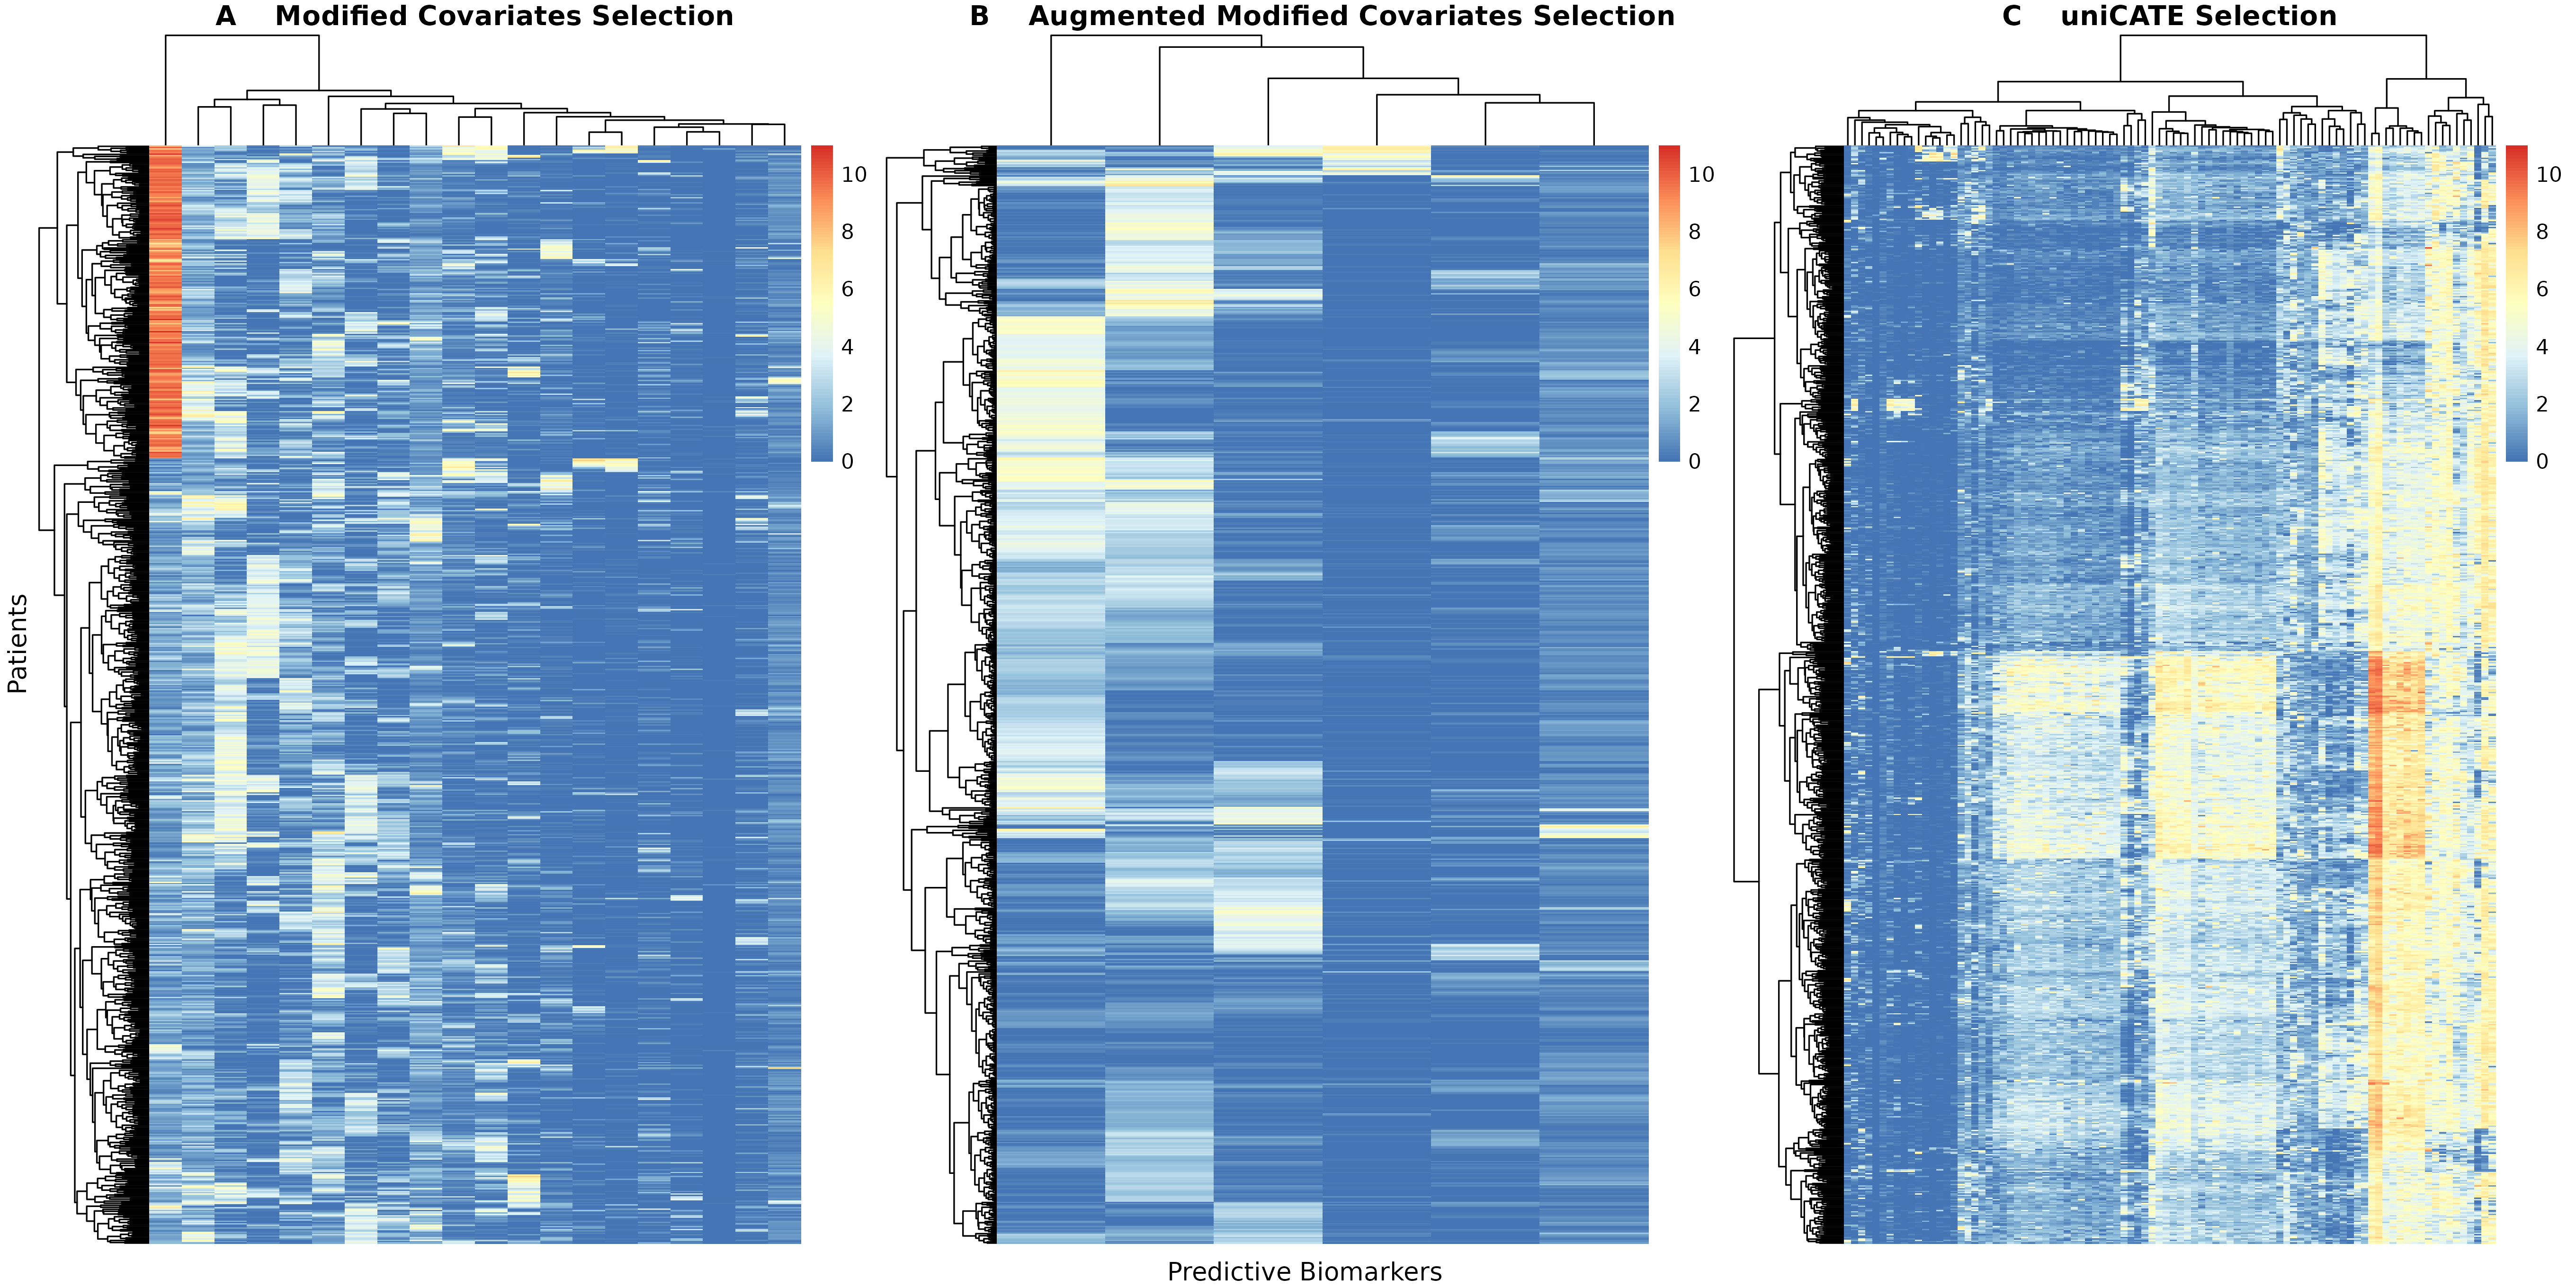
\includegraphics[width=0.295\textwidth]{figures/heatmaps.png}
      \end{tikzfigure}
    \end{center}
  }

  \myblock{Conclusion}{
    A one-sentence takeaway of your findings. Don't forget to include links or
    QR codes to your paper, preprint and/or software, if publicly available. QR
    codes should be placed in the \texttt{logos} folder. Don't forget to update
    the path to the QR code on line 32 of this TeX file.
  }
  
  \mysmallblock{Reference}{
    \vspace{-2em}
    \bibliographystyle{unsrtnat}
    \bibliography{refs}
    \vspace{-1em}
  }

\end{columns}

\end{document}
